%%%%%%%%%%%%%%%%%%%%%%%%%%%%%%%%%%%%%%%%%
% baposter Landscape Poster
% LaTeX Template
% Version 1.0 (11/06/13)
%
% baposter Class Created by:
% Brian Amberg (baposter@brian-amberg.de)
%
% This template has been downloaded from:
% http://www.LaTeXTemplates.com
%
% License:
% CC BY-NC-SA 3.0 (http://creativecommons.org/licenses/by-nc-sa/3.0/)
%
%%%%%%%%%%%%%%%%%%%%%%%%%%%%%%%%%%%%%%%%%

%----------------------------------------------------------------------------------------
%	PACKAGES AND OTHER DOCUMENT CONFIGURATIONS
%----------------------------------------------------------------------------------------

\documentclass[portrait,a0paper,fontscale=0.285]{baposter} % Adjust the font scale/size here

\usepackage{graphicx} % Required for including images
\graphicspath{{figures/}} % Directory in which figures are stored

\usepackage{amsmath} % For typesetting math
\usepackage{amssymb} % Adds new symbols to be used in math mode

\usepackage{booktabs} % Top and bottom rules for tables
\usepackage{enumitem} % Used to reduce itemize/enumerate spacing
\usepackage{palatino} % Use the Palatino font
\usepackage[font=small,labelfont=bf]{caption} % Required for specifying captions to tables and figures

\usepackage{multicol} % Required for multiple columns
\usepackage{bigints}
\usepackage{url}
\setlength{\columnsep}{1.5em} % Slightly increase the space between columns
\setlength{\columnseprule}{0mm} % No horizontal rule between columns

\usepackage{tikz} % Required for flow chart
\usetikzlibrary{shapes,arrows} % Tikz libraries required for the flow chart in the template

\newcommand{\compresslist}{ % Define a command to reduce spacing within itemize/enumerate environments, this is used right after \begin{itemize} or \begin{enumerate}
\setlength{\itemsep}{1pt}
\setlength{\parskip}{0pt}
\setlength{\parsep}{0pt}
}

%\definecolor{lightblue}{rgb}{0.145,0.6666,1} % Defines the color used for content box headers
\definecolor{lightblue}{rgb}{1,0.3333,0.3333} %not very 'light blue'

\begin{document}

\begin{poster}
{
headerborder=closed, % Adds a border around the header of content boxes
colspacing=1em, % Column spacing
bgColorOne=white, % Background color for the gradient on the left side of the poster
bgColorTwo=white, % Background color for the gradient on the right side of the poster
borderColor=lightblue, % Border color
headerColorOne=black, % Background color for the header in the content boxes (left side)
headerColorTwo=lightblue, % Background color for the header in the content boxes (right side)
headerFontColor=white, % Text color for the header text in the content boxes
boxColorOne=white, % Background color of the content boxes
textborder=roundedleft, % Format of the border around content boxes, can be: none, bars, coils, triangles, rectangle, rounded, roundedsmall, roundedright or faded
eyecatcher=true, % Set to false for ignoring the left logo in the title and move the title left
headerheight=0.1\textheight, % Height of the header
headershape=roundedright, % Specify the rounded corner in the content box headers, can be: rectangle, small-rounded, roundedright, roundedleft or rounded
headerfont=\Large\bf\textsc, % Large, bold and sans serif font in the headers of content boxes
%textfont={\setlength{\parindent}{1.5em}}, % Uncomment for paragraph indentation
linewidth=2pt % Width of the border lines around content boxes
}
%----------------------------------------------------------------------------------------
%	TITLE SECTION 
%----------------------------------------------------------------------------------------
%
{
\includegraphics[height=3em]{IITlogo.png}} % First university/lab logo on the left
{\bf\huge{\hspace{-1.5in}Hybrid Methods for Simulation \\ \hspace{-1.5in}of Muon Ionization Cooling Channels}\vspace{0.1em}} % Poster title
{{ \large{\hspace{-1.5in}J. Kunz, P. Snopok$^1$ \hspace{12pt} Illinois Institute of Technology \\\hspace{-1.5in}M. Berz, K. Makino \hspace{12pt}Michigan State University \\\hspace{-1.5in}$^1$ also at Fermi National Accelerator Laboratory \vspace{-0.4em}}}}
{
\includegraphics[height=6em]{MAPlogo.png}} % Second university/lab logo on the right

%----------------------------------------------------------------------------------------
%	Introduction
%----------------------------------------------------------------------------------------

\headerbox{Muon Ionization Cooling Experiment (MICE) Layout}{name=mice,column=0,row=0,span=2}{
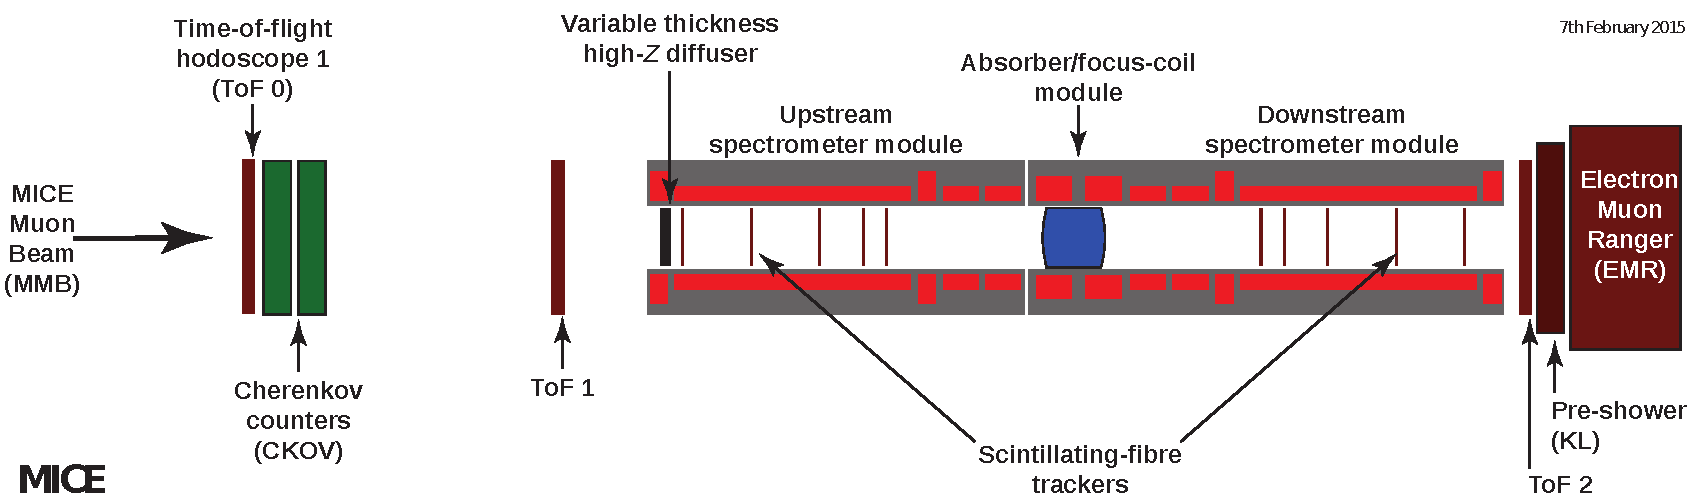
\includegraphics[width=\textwidth]{mice}
}

\headerbox{Absorbers}{name=absorbers,column=0,row=1,below=mice}
{
Talk about progress on absorbers, add pictures that illustrate agreement with other simulations (G4beamline, ICOOL), with data (MuScat) - all the usual stuff. This could possibly span more than one column if need be.
}

\headerbox{Magnetic coils}{name=coils,column=1,row=1,below=mice}
{
Talk about your recent tests with magnetic coils, show those figures with grids of particles, showing agreement when there only magnetic coils in the simulations.
}

\headerbox{Current challenges}{name=challenges,column=2,row=0}
{
Start by showing the layout of one of the cooling cells we are considering beyond MICE: with tilted coils and RF cavities clearly marked.
\mbox{} \\
The main challenge is once all of the individual elements were implemented and/or validated separately, we need to combine them into a single lattice and see how well they play together, and that work is currently underway.
\mbox{} \\
The other rather non-trivial thing to do in COSY is to implement tilted coils that are required in some configurations (see figure above).
}

\headerbox{Conclusions}{name=conclusions,column=2,row=2,below=challenges}
{
Summary...
}

\headerbox{References}{name=references,column=2,row=3,below=conclusions}
{
References...
}

\end{poster}

\end{document}